%%%%%%%%%%%%%%%%%%%%%%%%%%%%%%%%%%%%%%%%%%%%%%%%%%%%%%%%%%%%%%%%%%%%%%%%%%%%%%%%%%%%%%%%%%%%%%%%%%%%%%%
%%%%%%%%%%%%%% Template de Artigo Adaptado para Trabalho de Diplomação do ICEI %%%%%%%%%%%%%%%%%%%%%%%%
%% codificação UTF-8 - Abntex - Latex -  							     %%
%% Autor:    Fábio Leandro Rodrigues Cordeiro  (fabioleandro@pucminas.br)                            %% 
%% Co-autores: Prof. João Paulo Domingos Silva, Harison da Silva e Anderson Carvalho		     %%
%% Revisores normas NBR (Padrão PUC Minas): Helenice Rego Cunha e Prof. Theldo Cruz                  %%
%% Versão: 1.1     18 de dezembro 2015                                                               %%
%%%%%%%%%%%%%%%%%%%%%%%%%%%%%%%%%%%%%%%%%%%%%%%%%%%%%%%%%%%%%%%%%%%%%%%%%%%%%%%%%%%%%%%%%%%%%%%%%%%%%%%
\section{\esp Introdução}
Este artigo se trata de um atividade práticada da disciplina de Arquitetura de computador.Seguindo o artigo \cite{base}.

\section{\esp Conceitos}

A seguir serão mostrados alguns dispositivos de programação e seus respectivos conceitos.

\subsection{\esp ASICs}

ASIC é uma tecnologia com aplicações específicas o que as tornam aplicações mais caras e com um baixo reaproveitamento.

\subsubsection{\esp SPDLs}

SPLDs são uma categoria de dispositivos programaveis(Simple PLDs). Os PLDs(Programable Logic Device),por sua vez se trata de uma versão muito mais barata que às ASICs, pois se trata de um dispositivo que pode ser modificado após a fabricação pelo usuário e utiliza um máscaras mais genéricas,tornando seu desenvolvimento também mais barato.

\subsubsubsection{\esp CPDLs}
 
CPLDs se trata de um aglomerado de SPLDs(Complex PLDs).Devido a dificuldade do aumento da produtividade da arquitetura SPLD a solução encontrada foi adicionar vários blocos de SPLD em um estrutura programável surgindo assim os CPLDs.
 
 \subsubsubsubsection{\esp FPGA}
 
FPGA se trata de um grande arranjo de células configuráveis, e ao invés do uso do plano de portas OR ou AND ele utiliza células configuráveis ou blocos lógicos.

\section{\esp Diferenças}

A seguir sera mostrado uma tabela com as diferenças entre PROM,PLA e PAL:

\begin{figure}[ht]
	\centering	
	\caption[\hspace{0.1cm}Diferenças.]{Diferenças entre PROM,PLA e PAL}
	\vspace{-0.4cm}
	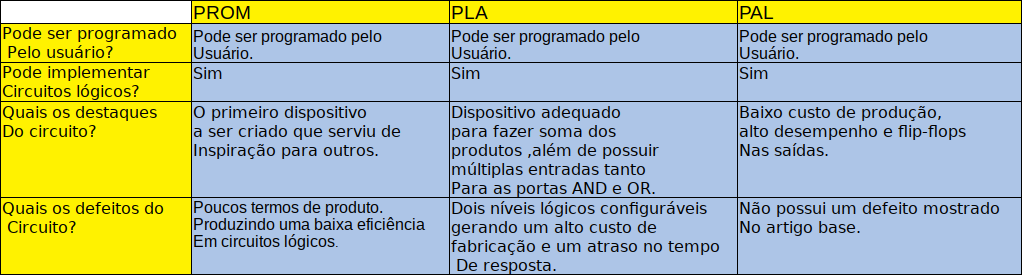
\includegraphics[width=1.0\textwidth]{figuras/dif.png}
	% Caption centralizada
% 	\captionsetup{justification=centering}
	% Caption e fonte 
	 \vspace{-0.2cm}
	\label{fig:figura1}
\end{figure}
\vspace{-0.5cm}

